\section{Principales técnicas de \textit{word embedding}}
\label{sec:techniques}

Como ya se ha indicado, los \textit{word embeddings} son modelos entrenados para
la obtención de representaciones vectoriales a partir de palabras. Estos modelos
pueden ser entrenados de forma individual para realizar su labor o como parte de
una tarea concreta de NLP, obteniendo unas representaciones más adaptadas al
problema específico~\cite{techniques}. De todas formas, un modelo ya entrenado
se puede reutilizar para tareas de NLP diferentes, pudiendo actualizarse para
adaptarse a las necesidades concretas de cada caso.

En las siguientes subsecciones se presentan y explican brevemente algunas de las
técnicas más conocidas de \textit{word embedding}.

\subsection{Word2vec}

Esta es una de las técnicas más conocidas y utilizadas. Se apoya en el
entrenamiento supervisado de una red neuronal para la obtención del
\textit{embedding}. En esta técnica se usa el contexto espacial de una palabra
(las palabras cercanas a ella en el texto) para obtener su representación
vectorial. Dependiendo del proceso, distinguimos dos métodos principales: CBOW y
\textit{skip-gram}.

\subsubsection{\textit{Continuous bag-of-words}}

El primer método es el de la bolsa de palabras común (CBOW por sus siglas en
inglés). En este método, se construye una red neuronal que toma como entrada las
palabras cercanas a la palabra objetivo e intenta predecir esta palabra
objetivo. El modelo de la red se puede ver en la Figura \ref{fig:cbow}, donde
$w(t)$ es la palabra objetivo y $w(t-2)$, $w(t-1)$, $w(t+1)$ y $w(t+2)$ son las
2 palabras anteriores y posteriores en el texto.

Se usa la codificación \textit{one-hot} de las palabras como entrada, usando
también esta codificación de la palabra objetivo para calcular la función de
pérdida de la salida obtenida durante el entrenamiento. De esta forma, en el
proceso de predecir la palabra objetivo, la red aprende la representación
vectorial de esta palabra. Como detalle, la capa oculta que posee esta red y que
se puede ver en la Figura no realiza activación, sino que sencillamente realiza
la suma ponderada de las entradas. En la capa de salida se usa una activación
\textit{softmax} para obtener el vector de la palabra objetivo, lo cuál supone
la única componente no lineal de la red. El aprendizaje de la red se realiza
mediante \textit{backpropagation}.

\begin{figure}
    \centering
    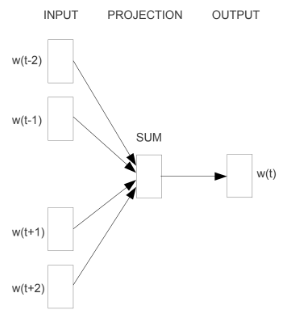
\includegraphics[width=0.6\textwidth]{images/word2vec/cbow.png}
    \caption{Modelo de red de CBOW}
    \label{fig:cbow}
\end{figure}

\subsubsection{\textit{Continuous skip-gram}}

Con el método CBOW, obtenemos las representaciones vectoriales de las palabras a
partir de su contexto. \textit{Skip-gram} se puede considerar como el método
inverso. En este caso, la entrada de la red es la codificación \textit{one-hot}
de la palabra cuya representación se desea obtener, y las salidas son $C$
distribuciones de probabilidad, una para cada palabra del contexto. Este modelo
se puede ver en la Figura \ref{fig:skip-gram} y, comparándolo con el modelo
de CBOW de la Figura \ref{fig:cbow}, observamos que, efectivamente, se trata de
la estructura inversa de este modelo.

\begin{figure}
    \centering
    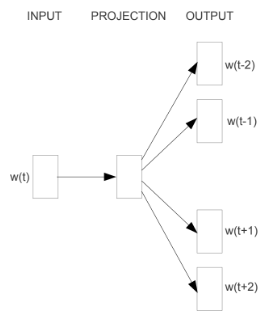
\includegraphics[width=0.5\textwidth]{images/word2vec/skip-gram.png}
    \caption{Modelo de red de \textit{skip-gram}}
    \label{fig:skip-gram}
\end{figure}

\subsection{GloVe}

El nombre de GloVe viene directamente de acortar las palabras \textit{global
    vectors}. Se trata de un algoritmo de aprendizaje no supervisado que trata
de ofrecer un enfoque diferente al de word2vec para la obtención de
representaciones vectoriales de palabras. El problema que los creadores de
GloVe encuentran en word2vec es que, a pesar de que su rendimiento no es
malo, se apoya exclusivamente en la información local del lenguaje, es
decir, en las palabras cercanas a una dada. Por el contrario, GloVe se basa
en las co-ocurrencias de palabras en todo el corpus, una estadística global,
para obtener los vectores de palabras.

En cuanto a su funcionamiento, GloVe no usa redes neuronales, sino que se trata
de un modelo basado en "conteo" (\textit{count-based model}). En el algoritmo de
GloVe, se empieza construyendo la matriz de co-ocurrencias del corpus. Para un
vocabulario de $N$ palabras, esta matriz $X$ es de tamaño $NxN$, guardando en
cada celda $X_{ij}$ el número de veces que las palabras $i$ y $j$ aparecen
juntas en el corpus. El algoritmo de GloVe realiza una reducción de la
dimensionalidad de esta matriz, pasando las columnas a ser las características
deseadas, de forma que cada celda $X_{ij}$ contiene el valor de la
característica $j$ para la palabra $i$. Cada palabra se ve entonces representada
por su vector de características.

Realmente, tanto word2vec como GloVe ofrecen resultados similares para tareas de
NLP. La diferencia más importante está en que es muy sencillo paralelizar la
implementación de GloVe, lo que permite entrenar el modelo con más datos de
forma más rápida.

\subsection{\textit{Embedding layer}}
\label{subsec:embedding-layer}

Esta última técnica consiste en añadir al principio de una red neuronal
encargada de realizar alguna tarea de NLP una capa que realice los \textit{word
    embeddings} específicamente. De esta forma, estos \textit{embeddings} se
aprenden de forma conjunta con el modelo de la red.

Las palabras entran a la red usando su codificación \textit{one-hot} y la
\textit{embedding layer} obtiene un vector de dimensión predefinida que
representa a cada una de ellas. Si la red es un perceptrón multicapa, estos
vectores obtenidos se concatenan antes de ser consumidos por el modelo de NLP.
Si, por el contrario, se usa una red neuronal recurrente, se pueden ir enviando
estos vectores de forma secuencial.

El principal problema de esta técnica es que requiere de una gran cantidad de
datos de entrenamiento y puede ser lenta, pero el resultado final es un
\textit{embedding} adaptado a la tarea de NLP específica que se desea realizar
y al texto que se posee.
